\section{Caratteristiche della rete aziendale}
L'ambiente in cui verrà installato un servizio VPN è illustrato nel diagramma seguente.
\subsection{Diagramma di rete}
\begin{figure}[h]
    \centering
    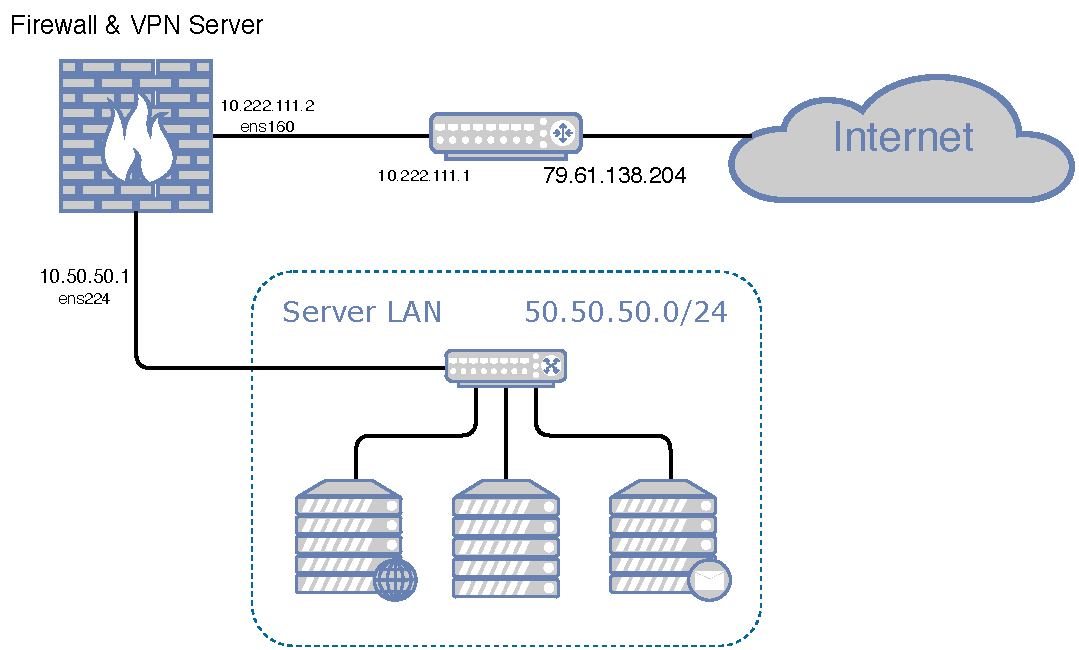
\includegraphics[width=14cm]{figure/networkDiagram.pdf}
    \caption{Diagramma di rete}
\end{figure}


\subsection{Descrizione dei componenti fondamentali}
Nei paragrafi seguenti verranno illustrati i componenti fondamentali di una rete aziendale.
\subsubsection{Router}
Un componente essenziale all'interno dell'infrastruttura di rete è il router. Il router è un dispositivo di rete che lavora al livello $3$ del modello OSI e che permette e gestisce l'instradamento dei pacchetti tra sottoreti diverse.
Le tabelle d'instradamento, salvate nella memoria interna del router, contengono informazioni che riguardano come raggiungere gli altri nodi della rete e sono lo strumento che permette al router di instradare correttamente i pacchetti.
Queste tabelle associano il prefisso IP~\cite[RFC0791]{RFC0791} e relativa maschera della sottorete di destinazione con il \emph{next-hop}, l'indirizzo IP del prossimo router a cui deve essere destinato al pacchetto affinché si avvicini alla sua vera destinazione, e l'interfaccia di rete del router da cui il pacchetto deve essere inoltrato affinché possa raggiungere il \emph{next-hop}.
Generalmente la funzione di routing è svolta da un componente hardware dedicato, che, se di fascia alta, permette di raggiungere prestazioni pari alla velocità della linea - ossia, spedisce i pacchetti alla stessa velocità alla quale li riceve.
Tuttavia, è possibile il compito venga svolto da server generici, a patto che siano dotati di un numero adatto di schede di rete, su cui gira un software apposito.

\subsubsection{Firewall}
In entrambi i casi, è comune che il router abbia un firewall \cite{RFC2979} integrato.
Un firewall è un dispositivo fisico, o un software, che ha come obiettivo la regolazione del traffico di una rete.
Ciò avviene applicando una serie di regole che coinvolgono lo stato, la porta e il protocollo dei pacchetti che lo attraversano.
L'amministratore di rete ha la responsabilità di inserire regole appropriate al contesto, affinché, tutto ciò che non è strettamente necessario, non venga fatto passare.
Un esempio di Firewall software molto conosciuto in ambienti UNIX, è \texttt{iptables}.
Il seguente comando mostra una regola che \emph{consente} il passaggio di un pacchetto in entrata sul firewall dalla scheda di rete \texttt{eth0}, destinato alla porta $22$ TCP, e che sia il primo di una comunicazione, o faccia parte di una comunicazione già instaurata.

\newpage
\texttt{
    iptables -A INPUT  -p tcp --dport 22 -i eth0 \linebreak
    -m state --state NEW,ESTABLISHED -j ACCEPT
}

Il sistema a disposizione avrà un router/firewall installato su un server, che ha come sistema operativo CentOS 7 \cite{CENTOS} - la versione gratuita di Red Hat Enterprise Linux \cite{RHEL}.

\subsubsection{Le reti locali utilizzate}
Nella configurazione della rete aziendale corrente è presente soltanto una sottorete, denominata LAN dei server, dove risiedono esclusivamente i server che erogano servizi all'esterno dell'azienda. Tutti i servizi per uso interno, destinati a una ulteriore LAN, in questo esempio sono erogati dal router/firewall stesso.

\subsection{Servizi offerti all'esterno}
L'azienda ha necessità di pubblicare
\begin{itemize}
    \item un sito web, il cui hosting è effettuato sul web server interno;
    \item un mail server, che si occupa di inviare e ricevere i messaggi di posta elettronica.
\end{itemize}
\noindent \textbf{Web servers}
Il sito web è servito in HTTP sulla porta $80$ e in HTTPS sulla porta $443$, e la pubblicazione è affidata a un noto servizio, \emph{Apache httpd} \cite{APACHE}.

\noindent \textbf{Mail servers}
L'azienda ha un mail server che si occupa di inviare, ricevere e archiviare i messaggi di posta dei dipendenti dell'azienda.

\subsection{Servizi offerti all'interno}
Per far sì che l'intero ecosistema funzioni, è necessario fornire alcuni servizi essenziali ai client della rete.
\subsubsection{DHCP server}
Il Dynamic Host Configuration Protocol \cite[RFC2131]{RFC2131} è un protocollo ausiliario che permette l'assegnazione automatica degli indirizzi IP e altri parametri di configurazione ai dispositivi connessi alla rete usando una architettura client-server.
Il DHCP offre un servizio non connesso e utilizza UDP come protocollo di trasporto. Il server ascolta le richieste (che saranno broadcast, destinate per convenzione all'indirizzo IP \texttt{255.255.255.255}) sulla porta $67$ UDP, e inoltra le risposte al client sulla porta $68$ UDP.
Altri parametri di configurazione che comunemente accompagnano l'appena assegnato indirizzo IP sono i server DNS \cite[RFC1034]{RFC1034} di default, l'indirizzo IP del default gateway, e la durata per il quale l'indirizzo IP assegnato è valido.

\subsubsection{DNS server}
Il Domain Name System (DNS) è il sistema di assegnazione gerarchico e decentralizzato dei nomi che identificano gli host in rete. Un'analogia che aiuta a comprendere la funzione del DNS è quella della rubrica telefonica.
Infatti, come nella rubrica telefonica viene mantenuta un'associazione tra un nome - facile da ricordare per una persona -  e il relativo numero di telefono - più difficile da ricordare, e facile da confondere -, così il DNS conserva dei \emph{resource records} composti da un nome - \texttt{example.com} - associato a un indirizzo IPv4 o IPv6 -  \texttt{93.130.23.53}.
Si tratta di un protocollo di livello $7$, che generalmente comunica sulla porta $53$ UDP, ma potrebbe sfruttare anche VPN o tunnel, TLS, HTTPS, Tor. È una potenzialità interessante, in quanto le richieste non sono criptate e si potrebbe andare incontro a problemi di sicurezza.
Il DNS è in grado di memorizzare anche altre informazioni riguardanti un certo dominio, tra cui:
\begin{itemize}
    \item i \emph{name servers} che sono autorità per quel dominio - coloro che a loro volta memorizzano i resource records dei vari sottodomini;
    \item gli indirizzi IP dei mail exchanger di riferimento per quel dominio;
    \item degli alias, ossia un'associazione tra due nomi di dominio.
\end{itemize}
Nella configurazione corrente, il server DNS, che gira sullo stesso server su cui è in esecuzione il Firewall, lavora come relay e il suo IP viene distribuito a tutti i client della rete interna via DHCP come DNS resolver.
Ciò significa che tutti gli host della rete, nel momento in cui devono risolvere un nome, inviano una richiesta al server DNS interno, che si occuperà lui di risolverlo e, una volta ottenuto il risultato, lo restituisce al richiedente.
\newpage
Questo comporta diversi vantaggi, tra cui:
\begin{itemize}
    \item la comunicazione verso l'esterno per la risoluzione dei nomi avviene da un unico punto della rete;
    \item si può fare caching, ossia mantenere in memoria per un certo periodo di tempo (che viene specificato nella risposta ricevuta dal server DNS) le risposte delle varie risoluzioni, cosicché, se di una richiesta si era già trovata la risposta, non dovrà essere fatta di nuovo la risoluzione;
    \item si possono implementare dei filtri per bloccare la risoluzione di nomi a cui si vuole limitare l'accesso;
    \item si possono facilmente tracciare le varie richieste.
\end{itemize}

\subsubsection{Altri servizi comunemente offerti}
\noindent \textbf{Web app interne.}
All'interno della rete locale dell'azienda, sono accessibili degli applicativi che permettono la gestione di alcuni sistemi, ad esempio degli apparati di rete.

\noindent \textbf{File servers.}
Affinché i dipendenti autorizzati possano collaborare e accedere a file condivisi, è stato predisposto un file server, a cui si può accedere con protocolli quali FTP \cite[RFC0791]{RFC0959} e SFTP. Tuttavia, i file in questione possono contenere dati sensibili. Per questo motivo, è necessario che la risorsa sia adeguatamente protetta, non esposta alla rete esterna e che l'accesso sia regolamentato.

\noindent \textbf{Database servers.}
Similmente al file server, c'è anche un database server a disposizione dei dipendenti, le cui necessità di sicurezza rispecchiano quelle del file server.

\noindent \textbf{Active Directory.}
Active Directory (AD) è un insieme di servizi di rete utilizzati dai sistemi operativi Microsoft. È fondato sui concetti di dominio (uno spazio in cui sono raggruppate tutte le risorse della rete, gli account utente, cartelle condivise, dispositivi in rete, etc) e di directory.
L'utilizzo di AD, e del suo sistema di autenticazione \emph{Kerberos}, è utile specialmente a realizzare il Single-Sign-On, un meccanismo attraverso il quale un utente, una volta effettuato il login nel dominio, ha accesso a tutti i servizi direttamente, senza dover effettuare login separati per ogni servizio.

\section{Necessità degli utenti}
Per quel che riguarda i dipendenti dell'azienda, hanno necessità di poter lavorare in modo autonomo da casa. Dunque devono poter accedere in maniera sicura a tutte le risorse disponibili all'interno della rete privata da qualsiasi parte del mondo.
\subsection{Remote work}
Lavorare da remoto è un qualcosa che sta prendendo sempre più piede nel mondo di oggi. Specialmente con la pandemia da Covid-19, si è visto come sia fondamenta offrire strumenti adeguati ai dipendenti per svolgere le proprie mansioni indipendentemente dalla loro posizione.
Tutto ciò, tuttavia, non deve avvenire a discapito della sicurezza.

\section{Requisiti di sicurezza}
Tra i requisiti principali di sicurezza, si ha: la possibilità di controllare il traffico, di avere una trasmissione sicura dei dati, di effettuare un controllo dei dispositivi aziendali.

\subsection{Controllo del traffico tramite proxy}
Un valido strumento per effettuare controllo del traffico e tenerne traccia tramite log è rappresentato dai proxy.
Un proxy è un server che si pone come intermediario tra la LAN interna e la rete esterna, generalmente per le comunicazioni che avvengono sulle porte TCP 21, 80 e 443, ossia quelle che utilizzano i protocolli FTP, HTTP e HTTPS.
Utilizzando un server proxy, i client, anziché comunicare direttamente con l'host di destinazione, inviano la richiesta al proxy, che si occupa di comunicare con l'host di destinazione e di restituire la risposta ottenuta all'iniziatore della richiesta.
Con questo tipo di intermediazione, è triviale registrare tutta l'attività che avviene e filtrare richieste ritenute non opportune.
Il filtraggio in questione è noto come URL filtering. Il funzionamento si basa su delle blacklist (o whitelist, nel caso inverso), contenenti URL a cui si vuole impedire ai client di accedere. Quando arriva una richiesta al server proxy, questa passerà e verrà inoltrata solo nel caso l'URL della richiesta non sia contenuto nella blacklist.

\subsection{Trasmissione sicura dei dati}
Come è possibile immaginare, per un'azienda è fondamentale poter contare su di un'infrastruttura che garantisca che i dati che transitano su di essa non vengano compromessi.

\subsubsection{Evitare intercettazioni}
Senza la garanzia di una trasmissione sicura dei dati, dove ``sicura'' si riferisce a tutte le diverse sfaccettature dell'ambito, si è esposti a ``eavesdropping attacks''. Questi attacchi consistono nell'ascoltare, senza farsi notare, le comunicazioni altrui, tramite strumenti di \emph{sniffing} posti a vari livelli.

Un'analogia esplicativa è quella delle \emph{cimici} posizionate all'interno dell'abitazione di un indagato, per registrare le sue comunicazioni.

\subsection{Controllo dei dispositivi}
L'azienda ha bisogno di poter controllare e gestire i dispositivi concessi in uso ai suoi dipendenti, affinché il software installato sia sempre e solo quello autorizzato, e le loro configurazioni siano quelle più adatte agli elevati standard di sicurezza richiesti.

\subsection{Compatibilità}
La soluzione finale deve garantire compatibilità con le ultime versioni dei tre sistemi operativi per desktop principali - macOS, Windows e le distribuzioni principali Linux -  e dei due sistemi operativi principali per mobile - iOS e Android.